\documentclass[11pt,a4paper]{article}
\usepackage[utf8]{inputenc}
\usepackage{gensymb}
\usepackage{graphicx}
\usepackage{amssymb}             
\usepackage{amsmath}    
\usepackage{amsfonts}
\usepackage{enumerate}
\usepackage{xcolor}
\usepackage{url}
\usepackage{listings}
\usepackage[top=2.5cm, bottom=2.5cm, left=2.7cm, right=2.7cm]{geometry} % Marges


\begin{document}


\begin{center}
\vspace{-3cm}
\Large{\textbf{ELEC0447 - Analysis of electrical power and energy systems}\\}
\bigskip
\Large{\textbf{Assignment: PandaPower project}\\}
\bigskip
\Large{\textbf{2021-2022}\\}

\end{center}



\section{Introduction}
This assignment aims to help you better understand the concepts seen during the course by illustrating them with a power flow tool and introducing some applications of power flow calculations for power system operation and planning.
You will use the Python library called Pandapower. The documentation of this library is here: \url{https://pandapower.readthedocs.io/en/v2.4.0/}. We also encourage you to check out the PandaPower channel on YouTube for video tutorials.

The assignment must be carried out by groups of \textit{three students} and submitted on Gradescope before \textbf{December 5 23:00}. You must submit 
\begin{enumerate}
\item a report named \verb|report_ELEC0447_2021.pdf| describing your results and analyses
\item the source code in Python as a single file named \verb|code_ELEC0447_2021.py|. We will automatically run your code to check it is working. You can import only the libraries \verb|pandapower|, \verb|pandas|, \verb|numpy|, and \verb|matplotlib| in your Python file.
\end{enumerate} 

You will also have to present your project with your report as support (preparing slides is unnecessary). Note that we will pay attention to how you present your results. Please make nice readable plots and give concise answers (expectations on the format and the length of the answers are provided below).


\section{Questions}
The assignment is divided in two parts. Along the assignment, we consider the IEEE 30-bus test system of Fig. \ref{fig:my_label}, that contains 41 lines, 5 generators and 20 loads \cite{Li2010}. In PandaPower, you can load this network with the provided Python function using the following command line:
\begin{lstlisting}
net = import_net()
\end{lstlisting}

\begin{figure}[ht!]
    \centering
    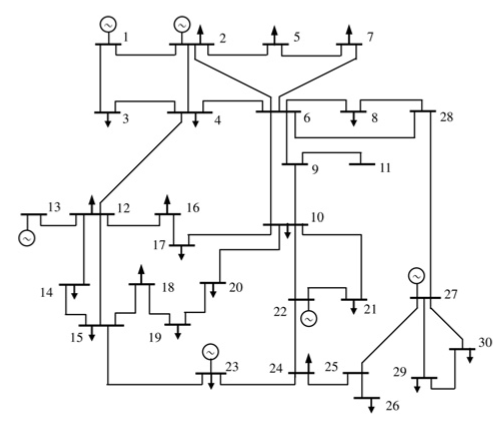
\includegraphics[scale=1]{ieee_30.png}
    \caption{IEEE 30-bus test system.}
    \label{fig:my_label}
\end{figure}

\subsection{Part 1}
Note that each question here must be solved independently, always starting from the initial power system (run import\_net() at the beginning of each question).\\
\textit{Expected: 5 pages, including figures.}

\begin{enumerate}
    \item Use PandaPower to run a power flow for this network\footnote{Do not forget to ensure that reactive limits for generators are enforced.}. Display the results with pf\_res\_plotly.py. What do you observe? Are all the voltages between the limits? Are the line loadings acceptable?\\
    \textit{Expected: 1 plot with the power flows, 1 bar graph with the voltage magnitudes at the different nodes.}
    
    \item Use the power flow tool to analyze the impact of a progressive increase of consumed power at bus 30\footnote{The index corresponding to bus 30 is 29 as the index starts at 0.}, while keeping the power factor at this node constant. In particular, look at the voltage magnitude of bus 30. At some point, the power flow will no longer converge. Why? For which amount of active power consumed? Plot the voltage magnitude of bus 30 with respect to the active power consumed at that bus. For this question, \textbf{do not enforce the reactive power limits of the generators.}\\
    \textit{Expected: 1 plot showing the voltage magnitude with respect to the power consumed.}
    
    \item Add a capacitor bank to bus 30 such that the power factor becomes 0.9 (leading)\footnote{You can also simply adapt the reactive power consumed at that bus to match the desired power factor.}. Increase the power consumed at bus 30 and analyze the results. For which amount of active power consumed does the power flow not converge? Plot the voltage magnitude of bus 30 with respect to the active power consumed at that bus. Compare the results you found with those of the previous question. For this question, \textbf{do not enforce the reactive power limits of the generators.}\\
    \textit{Expected: 1 plot with the voltage magnitude with respect to the power consumed.}
    
    \item Add a phase-shifter\footnote{You can choose as characteristics for this transformer: sn\_mva=400, vk\_percent=33.572608, vkr\_percent=0.92.} to prevent the overloading of the line between bus 6 and 8 (line 9). The phase-shifter should not induce overloading in other lines. Plot the loading of line 9 with respect to the phase shift imposed by your phase-shifter. The phase-shifter should be placed in series with the line where you consider to add it.\\
    \textit{Expected: 1 plot with the power flows after the addition of the phase-shifter, 1 plot of the loading of line 9 with respect to the phase shift.} 
       
    \item Convert bus 13 to a PQ node. Play with the reactive power Q injected into the grid. What is the impact on the network, regarding power flows and voltages?\\
    \textit{Expected: Figures showing the evolution of the power flows with different reactive powers Q.}
    
    \item Replace the existing line between bus 4 and bus 12 by a DC line. Consider a lossless DC line and play with the injected power and voltage magnitudes at both sides of the line. What is the impact on the power flows?\\
    \textit{Expected: Figures showing the evolution of the power flows with different injected power and modulated voltages.}
    
\end{enumerate}

\subsection{Part 2}
In this part, the IEEE 30-bus test system is used but the load data is different for each group. When you have your group, send an email to \url{antonin.colot@uliege.be} to receive your data, which consist of several CSV files describing the load active and reactive powers and the generator active powers and voltage magnitudes along the 24 hours of one day.\\
\textit{Expected: 5 pages, including figures.}

\begin{enumerate}
    \item Use the PandaPower Timeseries module to run a power flow along the 24 time steps. What do you observe?
    
    \item When power system operators operate the network, they usually ensure that the system will continue to operate, even in case of a loss of one of its elements. This is called the N-1 security criterion. Here we consider that the system is N-1 compliant if the voltage magnitudes and line loadings are within limits even in case of a loss of any one line in the system. 
    
    Based on your analysis at the previous question, select an hour of the day where you think problems could arise and check if your network is compliant with the N-1 criterion at that period, i.e. remove one line at a time and use the PandaPower Timeseries module with one time step to run the power flow and check if some line or bus voltage constraints are violated when that line is not in service. If the network is not N-1 compliant, which lines are problematic? What are the nature of the problems? Justify the choice of the time step studied.
    
    \item Let's imagine you have the possibility to realize an investment in the network to ensure that the line and bus voltage constraints are not violated during the hour studied. Consider one of the biggest problems you identified with the N-1 analysis at the previous question. Which element(s), among those seen in the course, would you add to the network and where to resolve the problem ? Describe your choices and justify. Analyze the results and show the impact of your decision on the power flows in the network. In particular, show how your solution improved the aforementioned problem and check that it does not create new problems for the lines that were not problematic in the N-1 analysis.
\end{enumerate}



\bibliographystyle{ieeetr}
\bibliography{my_bib}



\end{document}
